If you have opened the Caesar Perspective, there are some configurations left. Open Window-$>$Customise Perspective... .\\ Check the Caesar-Checkbox as shown below.\\\\
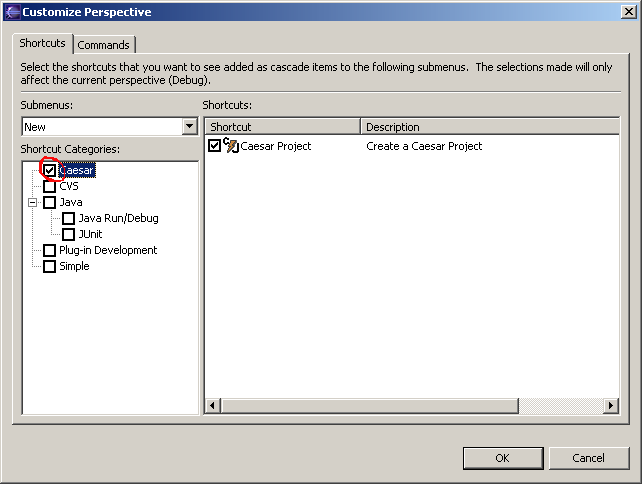
\includegraphics[width=0.80\textwidth]{images/propert.png}\\

If you have done this two new Buttons will appear in the Toolbar.\\\\

\includegraphics[width=0.90\textwidth]{images/toolbar.png}\newpage

With the "P"-Button the "Caesar-Configuration-Wizard" will be shown.\\\\
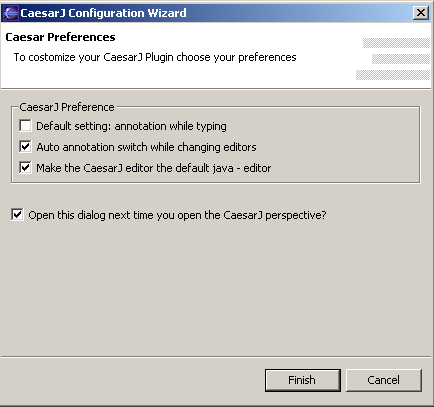
\includegraphics[width=0.80\textwidth]{images/view_properties.png}\\

The "A"-Button toggels the "Annotation-While-Typing" option on or off. Even for the Java-Editor!


